\documentclass{article}
\usepackage[utf8]{inputenc}
\usepackage{authblk}
\usepackage{setspace}
\usepackage[margin=1.25in]{geometry}
\usepackage{graphicx}
\graphicspath{{./figures/}}
\usepackage{subcaption}
\usepackage{amsmath,amssymb}
\usepackage{booktabs,longtable,array}
\usepackage{lineno}
\usepackage[hidelinks]{hyperref}
\usepackage{microtype}
\usepackage[style=nejm,citestyle=numeric-comp,sorting=none]{biblatex}
\addbibresource{references.bib}
\linenumbers
\onehalfspacing
% Generated by manuscript/generate_plant_phenomics_numbers.py; do not edit.
\newcommand{\ManualPoleXMLFiles}{12}
\newcommand{\ManualPoleImages}{61}
\newcommand{\ManualPoleAnnotations}{199}
\newcommand{\ManualPoleUsable}{172}
\newcommand{\ManualPoleUnusable}{27}
\newcommand{\SupportPoleLengthFt}{5}
\newcommand{\SupportPoleLengthCm}{152.4}
\newcommand{\FieldMarkIntervalIn}{35}
\newcommand{\FieldMarkIntervalsPerRow}{4}
\newcommand{\AdjacentRowSpacingIn}{140}
\newcommand{\PoleRepeatabilitySeries}{39}
\newcommand{\PoleRepeatabilityRows}{12}
\newcommand{\PoleRepeatabilityAnnotations}{172}
\newcommand{\PoleRepeatabilityMedianCV}{1.24}
\newcommand{\PoleRepeatabilityMedianCVLo}{0.78}
\newcommand{\PoleRepeatabilityMedianCVHi}{1.99}
\newcommand{\PoleRepeatabilityNinetiethCV}{3.65}
\newcommand{\PoleRepeatabilityBelowFive}{38}
\newcommand{\PoleRepeatabilityMaximumCV}{11.51}
\newcommand{\FieldN}{132}
\newcommand{\FieldPlants}{33}
\newcommand{\FieldRows}{12}
\newcommand{\FieldSingleBias}{2.64}
\newcommand{\FieldSingleMAE}{12.03}
\newcommand{\FieldSingleRMSE}{16.81}
\newcommand{\FieldBayesBias}{2.73}
\newcommand{\FieldBayesMAE}{10.97}
\newcommand{\FieldBayesRMSE}{15.81}
\newcommand{\FieldMAEGain}{1.06}
\newcommand{\FieldMAEGainLo}{-0.16}
\newcommand{\FieldMAEGainHi}{2.39}
\newcommand{\FieldBootstrapReplicates}{20,000}
\newcommand{\FieldEndpointN}{33}
\newcommand{\FieldEndpointSingleBias}{2.78}
\newcommand{\FieldEndpointSingleMAE}{14.45}
\newcommand{\FieldEndpointSingleRMSE}{19.44}
\newcommand{\FieldEndpointBayesBias}{6.17}
\newcommand{\FieldEndpointBayesMAE}{12.38}
\newcommand{\FieldEndpointBayesRMSE}{17.02}
\newcommand{\FieldEndpointGain}{2.08}
\newcommand{\FieldEndpointGainLo}{-1.47}
\newcommand{\FieldEndpointGainHi}{6.82}
\newcommand{\FieldAfterFirstN}{99}
\newcommand{\FieldAfterFirstPlants}{32}
\newcommand{\FieldAfterFirstRows}{12}
\newcommand{\FieldAfterFirstSingleMAE}{12.58}
\newcommand{\FieldAfterFirstBayesMAE}{11.14}
\newcommand{\FieldAfterFirstGain}{1.44}
\newcommand{\FieldAfterFirstGainLo}{-0.21}
\newcommand{\FieldAfterFirstGainHi}{3.26}
\newcommand{\FieldDates}{5}
\newcommand{\FieldCovered}{125}
\newcommand{\FieldCoverage}{94.7}
\newcommand{\FieldIntervalWidth}{75.4}
\newcommand{\FieldIntervalMedianWidth}{67.4}
\newcommand{\FieldCoveredEighty}{115}
\newcommand{\FieldCoverageEighty}{87.1}
\newcommand{\FieldCoverageEightyLo}{79.3}
\newcommand{\FieldCoverageEightyHi}{93.6}
\newcommand{\FieldIntervalWidthEighty}{47.9}
\newcommand{\FieldIntervalWidthEightyLo}{46.9}
\newcommand{\FieldIntervalWidthEightyHi}{49.4}
\newcommand{\FieldCoveredNinetyFive}{125}
\newcommand{\FieldCoverageNinetyFive}{94.7}
\newcommand{\FieldCoverageNinetyFiveLo}{89.4}
\newcommand{\FieldCoverageNinetyFiveHi}{98.6}
\newcommand{\FieldIntervalWidthNinetyFive}{75.4}
\newcommand{\FieldIntervalWidthNinetyFiveLo}{73.5}
\newcommand{\FieldIntervalWidthNinetyFiveHi}{78.3}
\newcommand{\FieldEndpointCovered}{31}
\newcommand{\FieldEndpointCoverage}{93.9}
\newcommand{\FieldEndpointIntervalWidth}{67.0}
\newcommand{\PixelImages}{30}
\newcommand{\PixelInstances}{150}
\newcommand{\PixelMatched}{149}
\newcommand{\PixelDetectionRate}{99.3}
\newcommand{\PixelHeightMAEPx}{29.5}
\newcommand{\PixelHeightBiasPx}{9.4}
\newcommand{\PixelHeightRMSECm}{15.91}
\newcommand{\PixelHeightMAECm}{12.27}
\newcommand{\PixelHeightBiasCm}{3.90}
\newcommand{\PixelHeightCorr}{0.837}
\newcommand{\PixelCmPerPx}{0.415886}
\newcommand{\PixelTopMAEPx}{28.3}
\newcommand{\PixelRootMAEPx}{18.2}
\newcommand{\PoleDevCameras}{6}
\newcommand{\PoleDevN}{1083}
\newcommand{\PoleDevMAEIn}{0.186}
\newcommand{\PoleDevMAELoIn}{0.156}
\newcommand{\PoleDevMAEHiIn}{0.218}
\newcommand{\PoleTestCameras}{3}
\newcommand{\PoleTestN}{427}
\newcommand{\PoleTestMAEIn}{0.208}
\newcommand{\PoleTestMAELoIn}{0.158}
\newcommand{\PoleTestMAEHiIn}{0.262}
\newcommand{\DownAllN}{2162}
\newcommand{\DownAllImages}{394}
\newcommand{\DownAllCameras}{10}
\newcommand{\DownAllBiasCm}{0.04}
\newcommand{\DownAllMAECm}{2.20}
\newcommand{\DownAllRMSECm}{5.37}
\newcommand{\DownAllCameraBiasCm}{0.58}
\newcommand{\DownAllCameraMAECm}{2.93}
\newcommand{\DownAllCameraRMSECm}{6.78}
\newcommand{\DownAllCameraMAELoCm}{1.86}
\newcommand{\DownAllCameraMAEHiCm}{4.64}
\newcommand{\DownOneBandN}{1110}
\newcommand{\DownOneBandImages}{394}
\newcommand{\DownOneBandCameras}{10}
\newcommand{\DownOneBandBiasCm}{0.07}
\newcommand{\DownOneBandMAECm}{1.46}
\newcommand{\DownOneBandRMSECm}{3.15}
\newcommand{\DownOneBandCameraBiasCm}{0.40}
\newcommand{\DownOneBandCameraMAECm}{1.91}
\newcommand{\DownOneBandCameraRMSECm}{3.95}
\newcommand{\DownOneBandCameraMAELoCm}{1.24}
\newcommand{\DownOneBandCameraMAEHiCm}{2.98}
\newcommand{\PoleDailyImages}{438}
\newcommand{\PoleDailyPassing}{376}
\newcommand{\AssembledImages}{391}
\newcommand{\AssembledRows}{2283}
\newcommand{\AssembledCameras}{9}
\newcommand{\AssembledPlants}{54}
\newcommand{\PoleStreamRows}{1686}
\newcommand{\PoleStreamForecasts}{1638}
\newcommand{\PoleStreamPlants}{48}
\newcommand{\PoleStreamCameras}{8}
\newcommand{\PoleStreamImages}{330}
\newcommand{\GuessedCoverage}{88.6}
\newcommand{\CalibratedCoverage}{96.4}
\newcommand{\GuessedWidth}{66.6}
\newcommand{\GuessedMedianWidth}{64.6}
\newcommand{\CalibratedWidth}{98.1}
\newcommand{\CalibratedMedianWidth}{93.8}
\newcommand{\ProcessHeightSD}{16.866}
\newcommand{\OutlierProbability}{0.0512}
\newcommand{\OutlierSD}{70.62}
\newcommand{\CalibrationIntervals}{1172}
\newcommand{\CalibratedWIS}{8.08}
\newcommand{\CalibratedLogScore}{-4.440}
\newcommand{\UncertaintyDevN}{1266}
\newcommand{\UncertaintyDevCameras}{6}
\newcommand{\UncertaintyDevPlants}{36}
\newcommand{\UncertaintyDevWIS}{7.93}
\newcommand{\UncertaintyTestN}{372}
\newcommand{\UncertaintyTestCameras}{2}
\newcommand{\UncertaintyTestPlants}{11}
\newcommand{\UncertaintyTestBias}{0.73}
\newcommand{\UncertaintyTestMAE}{15.58}
\newcommand{\UncertaintyTestRMSE}{22.89}
\newcommand{\UncertaintyTestWIS}{8.60}
\newcommand{\UncertaintyTestLogScore}{-4.486}
\newcommand{\UncertaintyDevCoverageFifty}{63.7}
\newcommand{\UncertaintyDevWidthFifty}{30.7}
\newcommand{\UncertaintyTestCoverageFifty}{65.1}
\newcommand{\UncertaintyTestWidthFifty}{30.6}
\newcommand{\UncertaintyDevCoverageEighty}{87.8}
\newcommand{\UncertaintyDevWidthEighty}{59.4}
\newcommand{\UncertaintyTestCoverageEighty}{86.3}
\newcommand{\UncertaintyTestWidthEighty}{59.3}
\newcommand{\UncertaintyDevCoverageNinety}{94.1}
\newcommand{\UncertaintyDevWidthNinety}{78.4}
\newcommand{\UncertaintyTestCoverageNinety}{92.7}
\newcommand{\UncertaintyTestWidthNinety}{78.2}
\newcommand{\UncertaintyDevCoverageNinetyFive}{96.8}
\newcommand{\UncertaintyDevWidthNinetyFive}{98.2}
\newcommand{\UncertaintyTestCoverageNinetyFive}{94.9}
\newcommand{\UncertaintyTestWidthNinetyFive}{97.8}
\newcommand{\UncertaintyTestMedianWidthNinetyFive}{94.2}
\newcommand{\ForecastBayesMAE}{15.13}
\newcommand{\ForecastBayesRMSE}{21.34}
\newcommand{\ForecastLastMAE}{16.64}
\newcommand{\ForecastLastRMSE}{23.63}
\newcommand{\ForecastLinearMAE}{19.95}
\newcommand{\ForecastLinearRMSE}{27.52}
\newcommand{\CausalPrefixes}{391}
\newcommand{\CausalRows}{51,035}
\newcommand{\CausalMismatches}{0}
\newcommand{\PriorNoneRMSE}{10.48}
\newcommand{\PriorPostRMSE}{8.61}
\newcommand{\PriorInsideRMSE}{6.01}
\newcommand{\PriorInsideReduction}{42.7}
\newcommand{\PriorSimulationPlants}{480}
\newcommand{\PriorSimulationScenarios}{8}
\newcommand{\PriorSpuriousProbability}{0.30}
\newcommand{\PriorTruthSelectionRate}{97.0}
\newcommand{\PriorNoneRMSELo}{9.84}
\newcommand{\PriorNoneRMSEHi}{11.13}
\newcommand{\PriorPostRMSELo}{8.07}
\newcommand{\PriorPostRMSEHi}{9.16}
\newcommand{\PriorInsideRMSELo}{5.47}
\newcommand{\PriorInsideRMSEHi}{6.57}
\newcommand{\PriorVsPostGain}{2.60}
\newcommand{\PriorVsPostGainLo}{2.00}
\newcommand{\PriorVsPostGainHi}{3.20}
\newcommand{\RealAuditN}{63}
\newcommand{\RealAuditCameras}{6}
\newcommand{\RealAuditTracks}{17}
\newcommand{\RealAuditAgreement}{100.0}
\newcommand{\RealAuditSingleMAE}{13.38}
\newcommand{\RealAuditPostMAE}{13.07}
\newcommand{\RealAuditPriorMAE}{13.07}
\newcommand{\RealAuditSingleRMSE}{18.01}
\newcommand{\RealAuditPostRMSE}{17.72}
\newcommand{\RealAuditPriorRMSE}{17.72}
\newcommand{\FieldEWMABias}{-9.78}
\newcommand{\FieldEWMAMAE}{14.98}
\newcommand{\FieldEWMARMSE}{20.16}
\newcommand{\FieldEWMAGain}{4.01}
\newcommand{\FieldEWMAGainLo}{1.48}
\newcommand{\FieldEWMAGainHi}{6.73}
\newcommand{\FieldMedianBias}{-12.15}
\newcommand{\FieldMedianMAE}{18.77}
\newcommand{\FieldMedianRMSE}{27.14}
\newcommand{\FieldMedianGain}{7.80}
\newcommand{\FieldMedianGainLo}{3.83}
\newcommand{\FieldMedianGainHi}{12.68}
\newcommand{\FieldHoltBias}{-8.09}
\newcommand{\FieldHoltMAE}{14.04}
\newcommand{\FieldHoltRMSE}{19.25}
\newcommand{\FieldHoltGain}{3.08}
\newcommand{\FieldHoltGainLo}{0.77}
\newcommand{\FieldHoltGainHi}{5.48}
\newcommand{\FieldGaussianBias}{2.74}
\newcommand{\FieldGaussianMAE}{11.62}
\newcommand{\FieldGaussianRMSE}{16.52}
\newcommand{\FieldGaussianGain}{0.66}
\newcommand{\FieldGaussianGainLo}{-0.43}
\newcommand{\FieldGaussianGainHi}{1.79}
\newcommand{\FrozenMatches}{1970}
\newcommand{\SequentialMatches}{2018}
\newcommand{\SequentialExtraMatches}{48}
\newcommand{\FrozenTrackDistance}{0.0396}
\newcommand{\SequentialTrackDistance}{0.0283}
\newcommand{\PosteriorRootChanged}{1963}
\newcommand{\SimulationScenarios}{9}
\newcommand{\SimulationPlantsPerScenario}{60}
\newcommand{\SimulationRMSEMin}{9.07}
\newcommand{\SimulationRMSEMax}{18.07}
\newcommand{\SimulationCoverageMin}{80.0}
\newcommand{\SimulationCoverageMax}{98.5}


\title{Bayesian Longitudinal Maize Height Estimation with Prior-Guided Image Analysis}

\author[1]{Haoming Wang}
\author[1,2]{Chong Wang}
\author[3,4,5]{Yawei Li}
\author[3,5]{Cheng-Ting Yeh}
\author[3,4,5]{Patrick S. Schnable}
\author[1,*]{Peng Liu}
\affil[1]{Department of Statistics, Iowa State University, Ames, Iowa, USA.}
\affil[2]{Department of Veterinary Diagnostic and Production Animal Medicine, Iowa State University, Ames, Iowa, USA.}
\affil[3]{Plant Sciences Institute, Iowa State University, Ames, Iowa, USA.}
\affil[4]{Interdepartmental Genetics and Genomics Graduate Program, Iowa State University, Ames, Iowa, USA.}
\affil[5]{Department of Agronomy, Iowa State University, Ames, Iowa, USA.}
\affil[*]{Address correspondence to: pliu@iastate.edu}
\date{}

\begin{document}
\maketitle

\begin{abstract}
Affordable longitudinal field phenotyping from fixed cameras is limited by ambiguous detections and uncertain pixel-to-centimeter calibration. Most pipelines analyze each image separately and apply a longitudinal model only after measurement extraction. We instead feed the Bayesian predictive state into current-image analysis: predicted position guides plant association, and the predicted height distribution can score competing top candidates before the measurement enters the longitudinal update. The resulting physically calibrated Bayesian longitudinal method uses a robust particle filter for plant-specific height and growth. With fixed settings, each update conditions only on images through time $t$ and returns an as-of height distribution. Held-out red pole bands evaluated calibration across cameras and years. Against 132 manual measurements from all 33 plants in 12 rows, mean absolute error decreased from 12.03 to 10.97 cm (paired reduction 1.06 cm; 95\% row-cluster bootstrap interval, -0.16 to 2.39). A Gaussian local-linear Kalman filter achieved 11.62 cm; its paired difference from the particle filter was uncertain (0.66 cm; -0.43 to 1.79). After centimeter scales were standardized, 2024-derived parameters gave 94.9\% coverage with a 97.8-cm mean 95\% width in 372 forecasts from a subject-disjoint 2025 cohort. In controlled ambiguity, prior-guided candidate scoring reduced latent-height root mean squared error from 10.5 to 6.0 cm, compared with 8.6 cm when filtering began after candidate selection; a matched real-image audit found no candidate conflict. The study supports affordable longitudinal phenotyping while locating the methodological innovation at the image-analysis decision itself.
\end{abstract}

\noindent\textbf{Keywords:} Bayesian longitudinal model; prior-guided image analysis; maize height; particle filter; stationary camera; uncertainty calibration

\section{Introduction}

Longitudinal plant-height trajectories describe growth rate, developmental timing, and response to environment more directly than a single mature measurement. Repeated manual measurement is costly and can disturb field plots, while fixed red-green-blue cameras can collect the same view throughout a season at comparatively low cost. Existing time-series phenotyping systems have produced useful growth curves in maize and other crops \cite{ge2016temporal,liang2018timeseries,wang2020functional}. The practical obstacle is that a camera produces pixels rather than a physical measurement. Canopy overlap, occlusion, wind, changes in illumination, and the transition from leaf tips to reproductive structures make the top and base of an individual plant ambiguous. A separate reference object can establish scale, but its geometry and usable range must be known. In a conventional two-stage pipeline, each image is reduced to a fixed measurement before the longitudinal model sees it; the downstream model cannot use earlier images to resolve the current image-level choice. A longitudinal method must also state exactly when information becomes available and how uncertainty changes as new images accumulate.

Several parts of this problem have been addressed separately. Time-lapse cameras with an in-scene scale can measure crop height, including operator-assisted rice measurements \cite{mano2017precise,manoigawa2017nondestructive}. Stereo and structured imaging can estimate canopy height accurately, but require additional hardware or controlled acquisition \cite{cai2018stereo,tabb2019cass}. Fixed-camera maize methods have pooled information across images, fitted nondecreasing growth curves, and used early images as labels for later overlapping plants \cite{guo2021kat4ia,guo2023sscnn}. Other field-maize pipelines reuse locations from earlier growth stages as seed points for later segmentation or use prior-stage maize positions to guide current time-series point-cloud segmentation and height extraction \cite{gao2022individual,li2023multisource}. These studies establish that temporal position information can guide later image analysis; they do not evaluate the same coupling of causal image analysis, physical calibration, and height-distribution updating studied here.

State-space models provide a formal way to carry information through time. Kalman and particle filters are standard tools for sequential estimation \cite{west1997bayesian,durbin2012time,gordon1993particle}. Particle filtering has been used for real-time rice-height estimation from Sentinel-1 images, and a recent Bayesian pattern-matching framework estimates daily rice height from satellite vegetation indices and sparse field measurements \cite{yang2022ricepf,shimda2026bayesianheight}. A Kalman tracker has also been combined with a maize seedling detector for counting \cite{li2022kalman}, while Bayesian adaptive sampling has been applied to affordable time-lapse germination phenotyping \cite{mercier2025bayesian}. Bayesian inference necessarily uses prior information, so the mere presence of a prior is not our novelty claim. The distinction is architectural: the predictive state from earlier images is fed back into analysis of the current image before its measurement is finalized. In the field implementation, the running plant-position state guides association and base-position refinement. The stronger branch lets the predicted height distribution choose among competing top candidates; it is evaluated in controlled simulation and a matched real-image audit. Thus \emph{prior-guided} modifies image analysis, while \emph{Bayesian longitudinal} describes the height-growth method that supplies and updates the predictive state.

The study integrates three elements for longitudinal field phenotyping. First, prior-guided image analysis uses the predictive longitudinal state during current-image association and candidate selection rather than only after a measurement has been chosen. Second, in-scene physical references and recorded camera geometry convert the selected image extent to centimeters, with separate definitions for 2021 camera-support poles and 2024--2025 red-band calibration poles. Third, sequential, outlier-robust Bayesian updating returns a plant-specific height-growth distribution and exact-mixture predictive intervals. Online operation is an as-of update: when a new image is appended, the algorithm analyzes the available image prefix and reports a measurement after processing that image; later observations join the pool only when they arrive. We evaluate held-out pole bands for calibration, human image annotations for detection and physical-reference auditing, simulated latent trajectories for candidate ambiguity, and all available 2021 plant-date field measurements for physical-height agreement.

\section{Results}

\subsection{Physical calibration and extrapolation}

The alternating-band experiment produced a camera-cluster mean absolute error of \PoleDevMAEIn{} in (95\% camera-bootstrap interval, \PoleDevMAELoIn{}--\PoleDevMAEHiIn{}) in 2024 development cameras and \PoleTestMAEIn{} in (\PoleTestMAELoIn{}--\PoleTestMAEHiIn{}) in locked 2025 cameras (Table~\ref{tab:calibration}; Figure~\ref{fig:calibration}). The locked interval overlaps the development interval, which argues against a large year-specific failure but does not establish equivalence with only three test cameras.

Correctly directed root extrapolation showed little aggregate signed bias but increasing dispersion with distance below the fitted bands. At 1 ft below the retained range, \DownOneBandN{} predictions from \DownOneBandCameras{} cameras had an unweighted camera-mean bias of \DownOneBandCameraBiasCm{} cm, mean absolute error of \DownOneBandCameraMAECm{} cm (95\% camera-bootstrap interval, \DownOneBandCameraMAELoCm{}--\DownOneBandCameraMAEHiCm{}), and root mean squared error of \DownOneBandCameraRMSECm{} cm. Across all 1--3-ft distances, unweighted camera-mean absolute error rose to \DownAllCameraMAECm{} cm (\DownAllCameraMAELoCm{}--\DownAllCameraMAEHiCm{}) and root mean squared error to \DownAllCameraRMSECm{} cm. One development camera contributed only five usable images and had much larger 3-ft error, visible in Figure~\ref{fig:calibration}; this is a failure condition rather than evidence for broadly reliable extrapolation.

\begin{figure}[htbp]
\centering
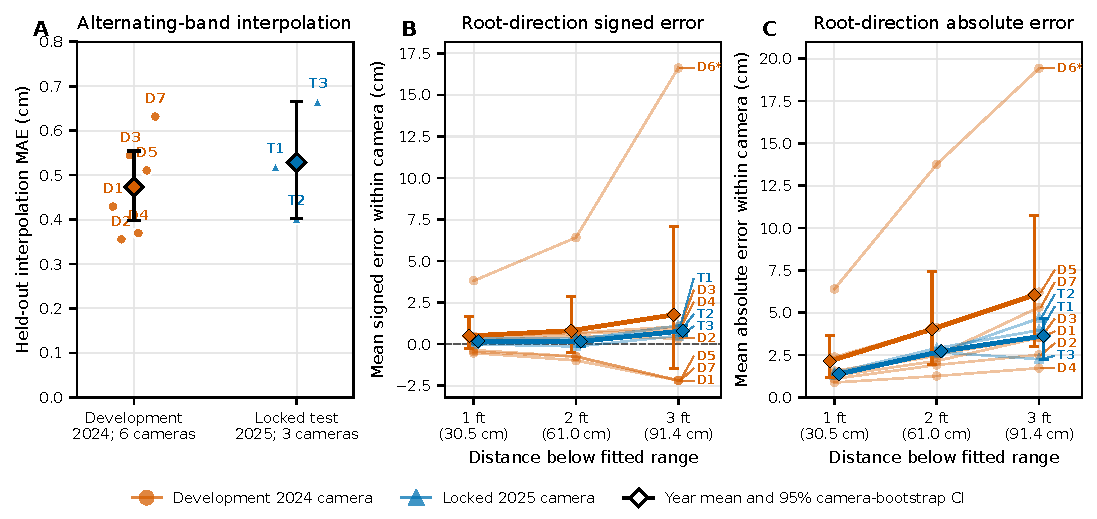
\includegraphics[width=\textwidth]{calibration_validation.pdf}
\caption{Camera-level physical-calibration validation. (a) Alternating-band interpolation mean absolute error for each 2024 development camera (D) and locked 2025 camera (T); diamonds and vertical intervals are unweighted year means and 95\% whole-camera bootstrap intervals. (b) Mean signed error and (c) mean absolute error when lower bands are dropped, the retained upper bands are fit, and positions 1--3 ft below the fitted range are predicted. Thin lines are cameras; thick lines and intervals are unweighted camera means and whole-camera bootstrap intervals. D6, marked with an asterisk, has only five usable images. Individual bands are automatic candidates; the inferential unit is the camera.}
\label{fig:calibration}
\end{figure}

\begin{table}[htbp]
\caption{Held-out calibration performance. Interpolation intervals resample whole cameras. Root-direction rows give unweighted means of camera-level error summaries from the correctly directed upper-to-lower experiment.}
\label{tab:calibration}
\centering
\begin{tabular}{lrrrrr}
\toprule
Experiment & Cameras & Predictions & Bias & MAE & RMSE \\
 & & & \multicolumn{3}{c}{Physical error} \\
\midrule
2024 alternating bands & \PoleDevCameras & \PoleDevN & -- & \PoleDevMAEIn{} in & -- \\
2025 alternating bands & \PoleTestCameras & \PoleTestN & -- & \PoleTestMAEIn{} in & -- \\
1 ft below fitted range & \DownOneBandCameras & \DownOneBandN & \DownOneBandCameraBiasCm{} cm & \DownOneBandCameraMAECm{} cm & \DownOneBandCameraRMSECm{} cm \\
1--3 ft below fitted range & \DownAllCameras & \DownAllN & \DownAllCameraBiasCm{} cm & \DownAllCameraMAECm{} cm & \DownAllCameraRMSECm{} cm \\
\bottomrule
\end{tabular}
\end{table}

\subsection{Prior-guided candidate selection}

In the controlled ambiguity experiment, the single-frame rule had plant-level height root mean squared error \PriorNoneRMSE{} cm (95\% plant-bootstrap interval, \PriorNoneRMSELo{}--\PriorNoneRMSEHi{}), and post-detection filtering reduced it to \PriorPostRMSE{} cm (\PriorPostRMSELo{}--\PriorPostRMSEHi{}). Allowing the predictive height distribution to score candidates before the update reduced it further to \PriorInsideRMSE{} cm (\PriorInsideRMSELo{}--\PriorInsideRMSEHi{}; Figure~\ref{fig:priorsim}). The paired reduction relative to post-detection filtering was \PriorVsPostGain{} cm (95\% interval, \PriorVsPostGainLo{}--\PriorVsPostGainHi{}). Prior-guided selection chose the truth-closest candidate \PriorTruthSelectionRate{}\% of the time. Benefits varied by simulated condition and were smallest when images were missing or growth plateaued early. This experiment establishes the candidate-choice mechanism under known ambiguity; it is not a claim that the same effect size occurred in the field data.

In the matched real-image audit, post-detection filtering and height-prior candidate scoring selected the same candidate in \RealAuditAgreement{}\% of \RealAuditN{} evaluated plant-dates. Their mean absolute errors were therefore identical at \RealAuditPostMAE{} cm, compared with \RealAuditSingleMAE{} cm for the single-frame candidate. The natural-image subset contained no candidate-choice conflict under the prespecified gates, so this audit is a negative control rather than evidence for a field accuracy gain from candidate re-ranking.

\begin{figure}[htbp]
\centering
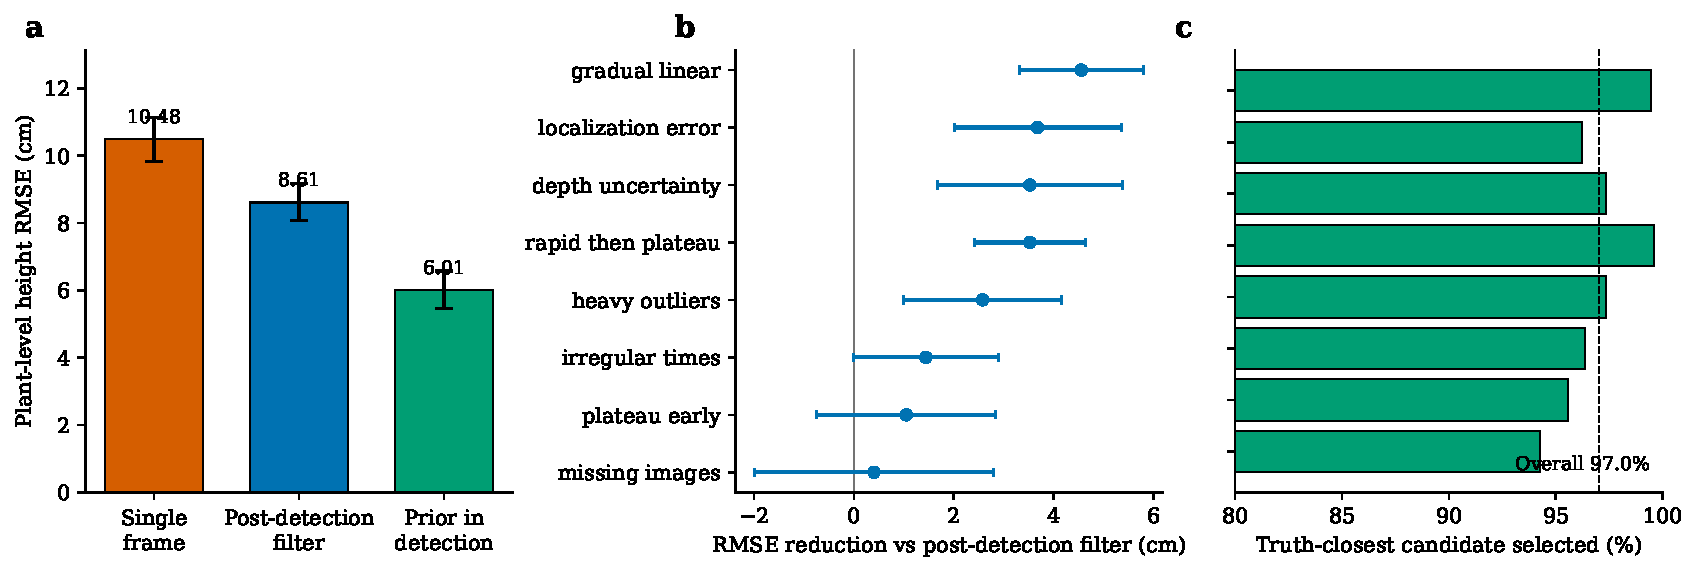
\includegraphics[width=\textwidth]{prior_in_detection_sim.pdf}
\caption{Controlled candidate-ambiguity experiment with \PriorSimulationPlants{} simulated plants across \PriorSimulationScenarios{} scenarios. (a) Mean plant-level root mean squared error with 95\% plant-bootstrap intervals. (b) Within-scenario reduction relative to post-detection filtering; points are means across 60 plants and bars are normal 95\% intervals across plants. Positive values favor prior-guided candidate selection. (c) Percentage of frames in which prior-guided scoring selected the candidate closest to the known latent height. Every method saw the same candidates and used the same state dynamics; only the location at which the prior acted differed.}
\label{fig:priorsim}
\end{figure}

\subsection{Predictive uncertainty transferred across years}

Exact mixture-based predictive evaluation materially changed the interpretation of uncertainty (Table~\ref{tab:uncertainty}). Guessed noise settings covered \GuessedCoverage{}\% of next image-derived measurements with a mean 95\% width of \GuessedWidth{} cm. After the depth correction was applied to every centimeter-scale noise quantity, the 2024-derived model covered \CalibratedCoverage{}\% with a \CalibratedWidth{}-cm mean width over the full stream. On the temporally later, subject-disjoint 2025 subset, coverage was \UncertaintyTestCoverageNinetyFive{}\% with a \UncertaintyTestWidthNinetyFive{}-cm mean width across \UncertaintyTestN{} forecasts from \UncertaintyTestPlants{} plant tracks and \UncertaintyTestCameras{} cameras. Its weighted interval score was \UncertaintyTestWIS{} cm. Plants were newly grown in 2025, so no biological subject recurred from the 2024 development cohort; repeated forecasts within each plant and camera remain dependent observations. Lower nominal levels remained conservative (Supplementary Figure S3), so the near-nominal 95\% result should not be interpreted as complete distributional calibration. The calibrated Bayesian predictive mean had mean absolute error \ForecastBayesMAE{} cm and root mean squared error \ForecastBayesRMSE{} cm, compared with \ForecastLastMAE{}/\ForecastLastRMSE{} cm for the last observation carried forward and \ForecastLinearMAE{}/\ForecastLinearRMSE{} cm for two-point linear extrapolation. These comparisons target the next noisy image measurement, not manual physical height.

The separate 2021 posterior intervals contained \FieldCovered{} of \FieldN{} manual heights (\FieldCoverage{}\%) and averaged \FieldIntervalWidth{} cm wide. The corresponding endpoint figures were \FieldEndpointCovered{} of \FieldEndpointN{} (\FieldEndpointCoverage{}\%) with a \FieldEndpointIntervalWidth{}-cm mean width. Reporting coverage and width together shows that agreement was obtained with substantial uncertainty.

\begin{table}[htbp]
\caption{Uncertainty evaluations with distinct targets. Predictive intervals are formed before the next image-derived measurement; posterior intervals are formed after the current 2021 image and compared with manual field height.}
\label{tab:uncertainty}
\centering
\small
\setlength{\tabcolsep}{4pt}
\begin{tabular}{p{3.0cm}p{3.5cm}rrrr}
\toprule
Target & Configuration & $n$ & Clusters & Coverage (\%) & Mean width (cm) \\
\midrule
Next image-derived measurement & Guessed noise, all years & \PoleStreamForecasts & \PoleStreamCameras & \GuessedCoverage & \GuessedWidth \\
Next image-derived measurement & 2024-derived, all years & \PoleStreamForecasts & \PoleStreamCameras & \CalibratedCoverage & \CalibratedWidth \\
Next image-derived measurement & 2025 held-out test & \UncertaintyTestN & \UncertaintyTestCameras & \UncertaintyTestCoverageNinetyFive & \UncertaintyTestWidthNinetyFive \\
2021 manual plant height & Posterior agreement interval & \FieldN & \FieldRows{} rows & \FieldCoverage & \FieldIntervalWidth \\
2021 manual endpoint height & Posterior agreement interval & \FieldEndpointN & \FieldRows{} rows & \FieldEndpointCoverage & \FieldEndpointIntervalWidth \\
\bottomrule
\end{tabular}
\end{table}

\subsection{Prefix updates reproduced exactly}

All \CausalPrefixes{} camera-time prefix recomputations matched the corresponding rows of the complete run, with \CausalMismatches{} mismatches among \CausalRows{} cumulative row comparisons. This verifies prefix invariance for the cached detection-to-measurement pipeline under fixed settings. It does not show that model development occurred prospectively, and it does not cover raw-image detector training. Sequential position updating associated \SequentialMatches{} detections, compared with \FrozenMatches{} under frozen first-frame anchors, and reduced mean normalized association distance from \FrozenTrackDistance{} to \SequentialTrackDistance{}. Because 2024--2025 manual plant heights are unavailable, these association results should be read as operational diagnostics rather than physical-height accuracy.

\subsection{Detector and field-height agreement}

Five-fold detector validation matched \PixelMatched{} of \PixelInstances{} human masks (\PixelDetectionRate{}\%). The top keypoint was more difficult than the root (mean errors \PixelTopMAEPx{} and \PixelRootMAEPx{} pixels). Predicted vertical extent had an error of \PixelHeightMAEPx{} pixels, corresponding under the recorded 2021 geometric scale to mean absolute error \PixelHeightMAECm{} cm, signed error +\PixelHeightBiasCm{} cm, and root mean squared error \PixelHeightRMSECm{} cm; correlation with human mask extent was \PixelHeightCorr{}. These values replace the earlier centimeter conversion that had been fit using field height. They measure agreement with a human mask extent, not an independently clicked agronomic collar.

Across all \FieldN{} 2021 field records, the single-frame image extent had signed error +\FieldSingleBias{} cm, mean absolute error \FieldSingleMAE{} cm, and root mean squared error \FieldSingleRMSE{} cm. The robust Bayesian posterior mean had corresponding values +\FieldBayesBias{}, \FieldBayesMAE{}, and \FieldBayesRMSE{} cm (Table~\ref{tab:field}; Figure~\ref{fig:field}). It had the lowest point-estimate error among the five fixed causal comparison methods. The paired mean-absolute-error reduction relative to the single frame was \FieldMAEGain{} cm (95\% row-cluster bootstrap interval, \FieldMAEGainLo{} to \FieldMAEGainHi{}), and relative to the Gaussian local-linear Kalman filter it was \FieldGaussianGain{} cm (\FieldGaussianGainLo{} to \FieldGaussianGainHi{}). Both intervals include zero, so the observed advantage over the strongest comparators is modest and uncertain at this pilot scale. At the last observation for each plant, mean absolute error changed from \FieldEndpointSingleMAE{} to \FieldEndpointBayesMAE{} cm; these endpoint values are secondary sensitivity results.

\begin{table}[htbp]
\caption{All-plants agreement with 2021 manual field height. Every method is causal in image order and uses fixed settings that were not tuned on manual height. The primary analysis includes every one of the \FieldN{} available plant-date records. Paired intervals in the text resample the \FieldRows{} field rows.}
\label{tab:field}
\centering
\begin{tabular}{lrrrr}
\toprule
Estimator & $n$ & Signed error (cm) & MAE (cm) & RMSE (cm) \\
\midrule
Single-frame image extent & \FieldN & +\FieldSingleBias & \FieldSingleMAE & \FieldSingleRMSE \\
EWMA ($\alpha=0.5$) & \FieldN & \FieldEWMABias & \FieldEWMAMAE & \FieldEWMARMSE \\
Running median (3 images) & \FieldN & \FieldMedianBias & \FieldMedianMAE & \FieldMedianRMSE \\
Holt level--trend & \FieldN & \FieldHoltBias & \FieldHoltMAE & \FieldHoltRMSE \\
Gaussian local-linear Kalman & \FieldN & +\FieldGaussianBias & \FieldGaussianMAE & \FieldGaussianRMSE \\
Robust Bayesian particle filter & \FieldN & +\FieldBayesBias & \FieldBayesMAE & \FieldBayesRMSE \\
\bottomrule
\end{tabular}
\end{table}

\begin{figure}[htbp]
\centering
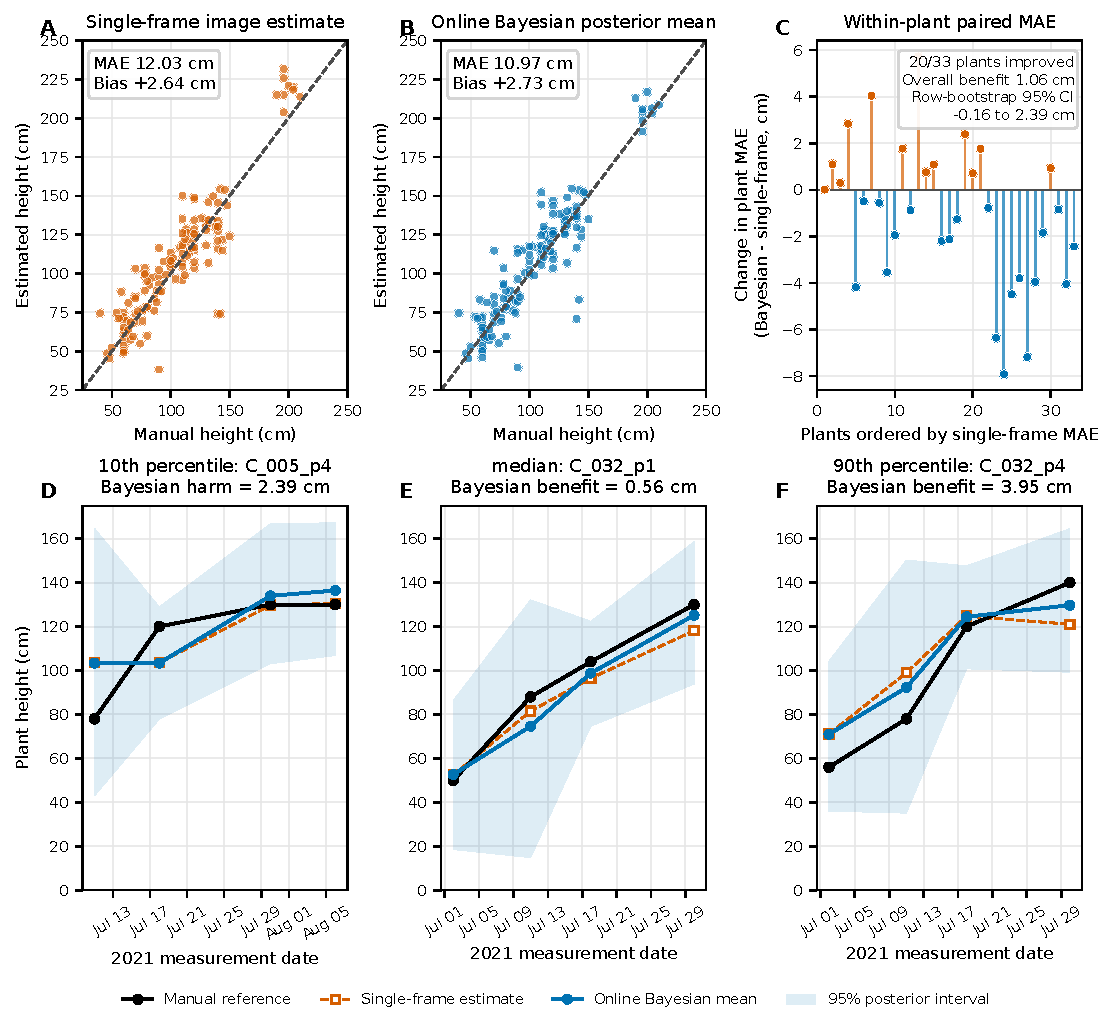
\includegraphics[width=\textwidth]{field_validation_2021.pdf}
\caption{All-plants 2021 field validation. (a,b) Single-frame and Bayesian estimates against manual height for all \FieldN{} records; dashed lines mark equality. (c) Within-plant difference in mean absolute error, ordered by single-frame error; negative values favor the Bayesian estimate. (d--f) Trajectories selected by the fixed 10th-, 50th-, and 90th-percentile rule on within-plant benefit, illustrating harm, median behavior, and benefit without residual-based exclusion. Shading is the 95\% latent-height posterior interval. The primary paired uncertainty is the row-cluster bootstrap interval reported in panel c and Table~\ref{tab:field}.}
\label{fig:field}
\end{figure}

\section{Discussion}

This study develops a physically interpretable route from an accumulating longitudinal fixed-camera image stream to an as-of plant-height distribution after each image. The key methodological contribution is feedback across the usual image/model boundary: the predicted longitudinal state participates in current-image analysis before a measurement is committed. A running position state informs association and base refinement, the stronger candidate branch lets the predicted height distribution score alternative top detections, physical references convert the selected extent to centimeters, and a robust particle filter updates plant-specific height, growth, and uncertainty. Prior field-maize systems have reused earlier locations for later segmentation and height extraction \cite{gao2022individual,li2023multisource}, and plant vision has used Kalman tracking \cite{li2022kalman}. Our contribution is the explicit prior-guided image-analysis loop inside a physically calibrated Bayesian longitudinal method, with separate evidence for each executed branch.

The evidence is strongest for component behavior and weakest for a large field accuracy gain. Held-out red-band interpolation transferred from six development cameras to three locked cameras with sub-inch error. The root-direction experiment also revealed why interpolation accuracy cannot be extrapolated casually: errors widened rapidly as the predicted point moved below the fitted band range, and one camera was particularly unstable. The candidate simulation showed that a height prior can prevent a confident but implausible candidate from entering the filter. The real-image audit, however, produced identical candidate choices for the two temporal methods. The height-prior candidate mechanism therefore remains demonstrated under controlled ambiguity rather than confirmed as a field advantage.

The all-plants 2021 comparison provides a realistic scale for the current longitudinal benefit. Mean absolute error decreased by about 1 cm relative to a single frame and by 0.66 cm relative to a Gaussian local-linear Kalman filter, but both row-cluster intervals included no improvement. The result does not support a claim that longitudinal Bayesian filtering uniformly improves height. It does show that the robust particle filter achieved the best point estimate across a broader set of causal baselines without manual-height tuning. All records are shown, errors are expressed in centimeters, and residual-based exclusions are absent from the primary analysis.

Uncertainty is similarly transparent. Applying the depth conversion to the observation, process, and outlier scales corrected a consequential unit mismatch. With parameters estimated from 2024 only, 95\% coverage was 94.9\% on the temporally later, subject-disjoint 2025 cohort with a 97.8-cm mean width, while 50\%, 80\%, and 90\% intervals overcovered. Coverage and sharpness together therefore describe a conservative distribution rather than proving perfect calibration. Repeated same-time images, direct uncertainty labels, or a hierarchical design are needed to separate measurement and biological variation and narrow intervals without losing coverage.

Several limitations determine the next experiments. First, the 2021 physical-height study contains only 33 plants in 12 rows, the 2025 interval test contains 372 forecasts from 11 plant tracks at two sequential cameras, and the calibration test contains three cameras. Second, annual replanting makes the 2025 cohort temporally later and subject-disjoint from 2024, which supports year-forward validation of calibration and next-image prediction. The 2024--2025 stream has no paired manual plant heights, however, while the 2021 comparison uses an archived segmentation extent and an externally learned growth field. The remaining gap is therefore end-to-end physical-height validation against manual measurements in a later subject-disjoint year, not subject overlap across years. Third, human validation serves component-specific purposes: 150 plant masks assess image extent, 132 field measurements assess physical height, and Haoming Wang's \ManualPoleAnnotations{} manual traces across \ManualPoleImages{} images audit the 2021 physical-reference geometry. These sources do not estimate inter-reader variation for agronomic landmarks. Fourth, the depth ratio assumes known distances, level ground, negligible roll, and stable camera geometry. Fifth, the released checkpoint permits inference on the curated images, but its complete original training provenance remains only partially documented.

A publication-scale extension should freeze the detector, physical calibration, growth field, noise settings, and candidate gates using one or more early development years; validate without retuning on one or more later, newly planted subject-disjoint cohorts with paired manual plant and physical-reference measurements; compare prior-in-image selection with the same detector followed by post-hoc filtering; and report plant-, camera-, or row-cluster intervals appropriate to the sampling design. The present 2024-to-2025 split already supplies temporal, subject-disjoint validation for calibration and next-image prediction; the extension would add later-year manual height validation.

\section{Materials and Methods}

\subsection{Experimental and technical design}

Figure~\ref{fig:workflow} shows the information flow. Let $\mathcal I_{\leq t}$ be the images available through acquisition time $t$. The image arriving at $t$ is appended to this pool, and the predictive state from $t-1$ is returned to the image-analysis stage before the current measurement is fixed. The running position state guides association; in the stronger branch, the propagated height distribution scores competing top candidates. Selected top and base rows are converted to centimeters, incorporated into the Bayesian longitudinal update, and returned as an as-of height distribution. An image acquired after $t$ is absent from this computation. This is the operational meaning of \emph{online} used throughout the paper. The available data were analyzed retrospectively, so we call the evaluation a retrospective validation of a prefix-causal algorithm rather than a historical prospective deployment. Hyperparameters and growth-field estimates must be frozen from development or external data before future prospective use.

\begin{figure}[htbp]
\centering

\includegraphics[width=\textwidth]{online_bayesian_workflow.pdf}
\caption{Workflow for the as-of image update. The feedback arrows place prior information inside current-image analysis: the running position state guides detection association and base refinement, and the dashed amber branch uses the predicted height distribution to choose among alternative top candidates. Solid blue stages were executed in the field pipeline; the height-candidate branch was evaluated in controlled simulation and the matched real-image audit. At time $t$, only $\mathcal I_{\leq t}$ is available; with settings fixed, a later image starts a new update and does not alter an earlier output.}
\label{fig:workflow}
\end{figure}

The study contains linked data sets with different roles (Table~\ref{tab:design}). The 2024 development and 2025 locked-test pole images evaluate calibration. A quality-controlled subset also supplies a daily image-derived plant stream for prequential uncertainty checks. Plants were newly grown in each season, so no biological plant subject recurs from the 2024 development cohort to the temporally later 2025 test cohort. The split is therefore subject-disjoint as well as year-forward, although repeated images within a plant and camera remain dependent. The 2021 field data provide manual heights on five dates and an archived single-frame segmentation extent for all available plant-date records. A separate set of 2021 human-annotated images supports out-of-fold detector validation. Haoming Wang's 2021 support-pole annotations provide a completed human audit of the physical installation; they are not treated as the red-band calibration poles.

\begin{table}[htbp]
\caption{Data sources, physical references, and inferential roles. Counts are reported at the unit used in each analysis.}
\label{tab:design}
\centering
\small
\begin{tabular}{p{2.1cm}p{3.0cm}p{4.2cm}p{4.1cm}}
\toprule
Data set & Units & Physical or annotation reference & Role \\
\midrule
2021 field heights & \FieldN{} records; \FieldPlants{} plants; \FieldRows{} rows; \FieldDates{} dates & Manual height and geometrically scaled image extent & All-plants physical-height agreement \\
2021 detector set & \PixelImages{} images; \PixelInstances{} masks & Highest and lowest pixels of each human mask & Five-fold out-of-image detection agreement \\
2021 support poles & \ManualPoleXMLFiles{} XML files; \ManualPoleImages{} retained images; \ManualPoleAnnotations{} human traces & Nominal \SupportPoleLengthFt{}-ft support pole; ground contact to camera mount/optical-center height & Human physical-reference and installation audit \\
2024 pole development & 7 installed cameras; \PoleDevCameras{} usable in held-out validation & Red bands spaced 1 ft edge-to-edge & Calibration development and noise estimation \\
2025 locked test & 3 installed and usable calibration cameras & Same red-band definition & Locked cross-camera/year calibration test \\
Quality-controlled sequential stream & \PoleStreamRows{} records; \PoleStreamPlants{} tracks; \PoleStreamCameras{} cameras; \PoleStreamImages{} images & Red-band calibration and camera geometry & Next-image prediction and interval evaluation \\
Candidate-ambiguity simulation & \PriorSimulationPlants{} plants in \PriorSimulationScenarios{} scenarios & Known latent height and correct candidate & Mechanism comparison with plant-cluster inference \\
\bottomrule
\end{tabular}
\end{table}

\subsection{Physical references and geometry}

Haoming Wang manually annotated the 2021 physical references in CVAT. The XML files contain labels \texttt{pole1} through \texttt{pole4}; each label identifies a different stationary-camera support pole visible in that image, and the number does not encode depth. The annotated vertical segment runs from ground contact to the nominal camera mounting or optical-center height, \SupportPoleLengthFt{} ft (\SupportPoleLengthCm{} cm). The field records also contain four horizontal layout intervals of \FieldMarkIntervalIn{} in, totaling \AdjacentRowSpacingIn{} in between adjacent rows. These horizontal marks are not tick marks on the support poles. The confirmed duplicate \texttt{C-039\_2021-07-30JPG.JPG} was removed while \texttt{C-039\_2021-07-30.JPG} was retained. The completed human audit contains \ManualPoleAnnotations{} traces on \ManualPoleImages{} unique XML-referenced images: \ManualPoleUsable{} marked usable and \ManualPoleUnusable{} marked unusable (Figure~\ref{fig:supportpole}).

\begin{figure}[htbp]
\centering
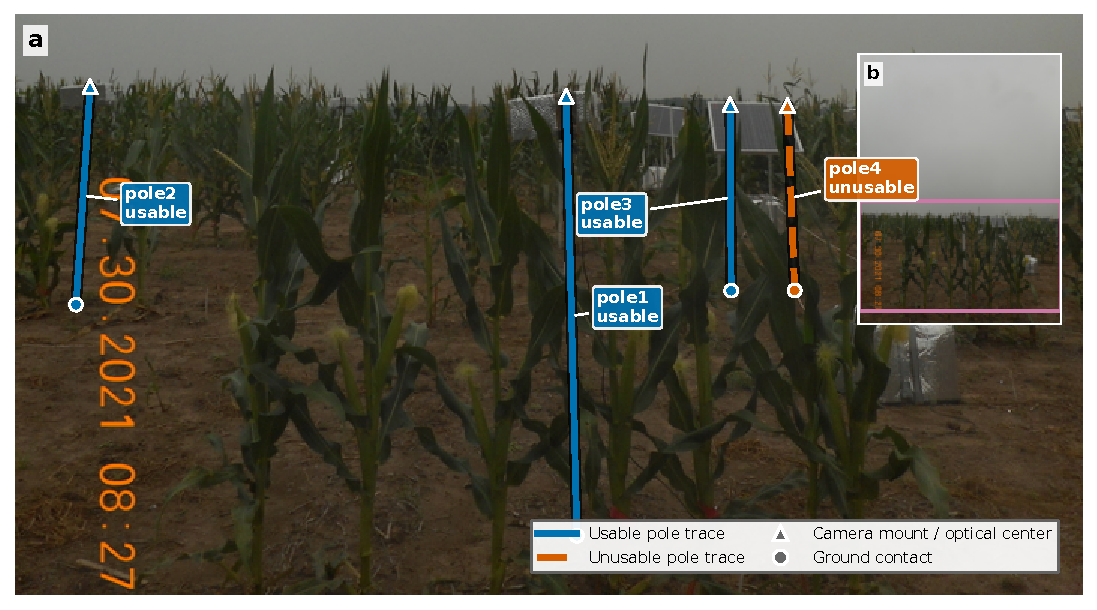
\includegraphics[width=\textwidth]{pole_annotation_2021.pdf}
\caption{Representative 2021 camera-support-pole annotations in \texttt{C-039\_2021-07-30.JPG}. Blue traces were marked usable and the orange trace unusable in the source XML. Circles denote ground contact and triangles the nominal camera mounting or optical-center height. Each traced support pole has a documented physical length of \SupportPoleLengthCm{} cm. The inset shows the full retained image and crop boundary. The \FieldMarkIntervalIn{}-in field marks recorded for this installation describe horizontal row layout and are not vertical pole graduations.}
\label{fig:supportpole}
\end{figure}

The 2024--2025 reference is a different object: an approximately 8--10-ft vertical calibration pole with red bands separated by 1 ft (30.48 cm), measured edge-to-edge. Its visible bottom is not assumed to be ground. Candidate band rows $y_j$ are assigned relative heights $z_j$, and a projective map is fit within each accepted reference image,
\begin{equation}
z(y)=\frac{a u+b}{c u+1}, \qquad u=\frac{y-\bar y}{s_y}.
\label{eq:calibration}
\end{equation}
Fits are rejected for insufficient bands, excessive line or height residuals, irregular spacing, nonmonotonicity, or a near-singular denominator. Because plant height is the difference between the mapped top and base rows, the arbitrary height datum cancels.

Recorded 2024--2025 geometry gives a camera height of 5.0 ft, camera-to-plant-row distance $D_{\mathrm{tgt}}=8.5$ ft, and camera-to-reference distance $D_{\mathrm{ref}}=10.0$ ft. Under a pinhole camera, negligible roll, and a shared level ground plane,
\begin{equation}
y-y_{\mathrm{horizon}}=f_{\mathrm{px}}\frac{H-z}{D}.
\label{eq:pinhole}
\end{equation}
Subtracting Equation~\ref{eq:pinhole} at the top and base shows that an extent calibrated at the pole depth is converted to the target depth by
\begin{equation}
h_{\mathrm{target}}=\frac{D_{\mathrm{tgt}}}{D_{\mathrm{ref}}}h_{\mathrm{pole}}=0.85h_{\mathrm{pole}}.
\label{eq:depth}
\end{equation}
Equation~\ref{eq:depth} is exact under the stated projection assumptions; uncertainty in distance, tilt, relief, lens distortion, wind, and maintenance remains empirical error. The 2021 single-frame height uses the separately documented camera geometry, 10.25 ft to the target row with a 4.5-mm focal length, 6.17-mm sensor width, and 1030-pixel stored field of view, giving \PixelCmPerPx{} cm/pixel with zero intercept.

\subsection{Prior-guided image analysis within the Bayesian longitudinal method}

For the 2024--2025 stream, a YOLOv8-pose model produces candidate plant instances with top and root keypoints. The first complete frame initializes six left-to-right tracks. At each later frame, observed root positions are matched to running track positions by minimum total horizontal distance, subject to a maximum normalized distance of 0.16. The track position and root row are then updated with a fixed gain of 0.5. This is prior-guided image analysis because the state carried from preceding images participates in current-image association and base refinement before the physical measurement is constructed. The sequential configuration associated \SequentialMatches{} detections and recovered \SequentialExtraMatches{} associations relative to frozen first-frame anchors; it changed the root used in the physical extent for \PosteriorRootChanged{} matched records. The position recursion has the form of an exponentially weighted moving average, or a steady-state Kalman update with fixed gain. The deployed assembler does not estimate position covariance and is not a fully Bayesian neural network.

The 2021 all-plants comparison uses the archived per-image segmentation extent \texttt{height\_sam}, multiplied by the recorded geometric scale. Manual field height is used only for scoring. The separate detector validation derives two keypoints from each human mask: the uppermost plant pixel and the lowermost plant pixel. This is an operational mask-extent definition, not an independently annotated flag-leaf collar. Five image-level folds were formed; a YOLOv8n-pose model was trained for 100 epochs on the other folds and evaluated on images that did not contribute to its training.

The height-prior candidate component isolates the same architectural question at the plant-top decision. Each current image in the simulation supplied one correct candidate with Gaussian error and, with probability \PriorSpuriousProbability{}, a competing high-confidence candidate displaced 25--60 cm upward or downward. Three estimators saw identical candidate sets: the highest-confidence single-frame candidate; the same independently selected candidate stream followed by a particle filter; and prior-guided image selection, which maximized detector confidence times the longitudinal predictive height density before filtering. The comparison therefore changes where the prior acts, not whether the downstream model is Bayesian. A complementary real-image audit used the same cached YOLO candidates, fixed geometric scale, association gates, and downstream particle filter for both temporal methods. Human-mask root positions initialized tracks only in the first available image, and manual field heights were used only for scoring. This audit comprised \RealAuditN{} plant-dates from \RealAuditTracks{} tracks and \RealAuditCameras{} cameras.

\subsection{Bayesian filtering of longitudinal height and growth}

We use \emph{filtering} in the state-space sense: after image $t$ is processed, the target is $p(h_t,r_t\mid Y_{1:t})$, the current height-growth distribution conditional on measurements available through $t$. This is distinct from spatial image filtering or denoising and from retrospective smoothing, which would use later measurements $Y_{t+1:T}$ to revise an earlier state.

For a plant observed at irregular interval $\Delta_t$, the latent height $h_t$ and growth rate $r_t$ follow
\begin{align}
h_t &= h_{t-1}+\Delta_t r_{t-1}+\eta_t, & \eta_t&\sim N(0,\sigma_h^2\Delta_t), \\
r_t &= r_{t-1}+\zeta_t, & \zeta_t&\sim N(0,\sigma_r^2\Delta_t),
\label{eq:state}
\end{align}
with $h_t$ truncated to $[0,450]$ cm and $r_t$ to $[-4,15]$ cm/day. The lower growth bound permits short apparent decreases rather than forcing an irreversible monotone ratchet. The image-derived measurement $Y_t$ has a robust two-component likelihood,
\begin{equation}
p(Y_t\mid h_t)=(1-\pi)\,\phi(Y_t;h_t,\sigma_t^2)+\pi\,\phi(Y_t;h_t,\sigma_{\mathrm{out}}^2),
\label{eq:mixture}
\end{equation}
where $\sigma_t$ combines a base pose term, pole-fit residual, out-of-range distance, and band-regularity term. A bootstrap particle filter with 5000 particles propagates, weights, and resamples the state when effective sample size falls below half the particle count \cite{gordon1993particle}.

Two interval targets are kept separate. A posterior interval summarizes uncertainty in latent height after image $t$ has been incorporated. A one-step predictive interval is formed before $Y_t$ is observed and targets the next image-derived measurement. If predicted height particles are $h_t^{(m)}$ with weights $w_m$, its cumulative distribution is
\begin{equation}
F_t(y)=\sum_m w_m\left[(1-\pi)\Phi\!\left(\frac{y-h_t^{(m)}}{\sigma_t}\right)+\pi\Phi\!\left(\frac{y-h_t^{(m)}}{\sigma_{\mathrm{out}}}\right)\right].
\label{eq:predictive}
\end{equation}
The 0.025 and 0.975 quantiles are obtained by numerical inversion of Equation~\ref{eq:predictive}. This replaces the earlier Gaussian variance approximation, which did not preserve the outlier-mixture tails.

The daily 2024 development increments set $\sigma_h=\ProcessHeightSD{}$ cm/$\sqrt{\mathrm{day}}$, $\pi=\OutlierProbability{}$, and $\sigma_{\mathrm{out}}=\OutlierSD{}$ cm from a robust median/median-absolute-deviation core-tail split over \CalibrationIntervals{} within-track intervals. Height, measurement standard deviation, process scale, and outlier scale are all expressed after the same 0.85 pole-to-target depth conversion. These values combine process and measurement variation because one observation per plant-time cannot identify those components separately. A comparison run retains the prespecified guessed values 1.5 cm/$\sqrt{\mathrm{day}}$, 0.08, and 60 cm, also expressed in target-row units. No 2025 observation enters the empirical noise estimates, and no 2025 plant subject appears in the 2024 development data.

For the 2021 external field comparison, the per-image observation standard deviation ranges from 12 to 30 cm with recorded daily wind, and the process-height scale is estimated from image increments without manual height. A nonparametric growth-rate field $\hat r(h)$ is learned from 2024--2025 pole-stream increments and transferred to 2021. No 2021 manual height enters the single-frame measurement, growth field, filter, or noise parameters. This use of later-year development data makes the 2021 exercise a retrospective physical-height benchmark rather than the year-forward validation; each 2021 update remains prefix-causal within its image sequence. The explicit early-to-late evaluation is the 2024 development to subject-disjoint 2025 test split.

\subsection{Validation and statistical analysis}

Physical calibration was evaluated by fitting alternating 1-ft automatically detected red bands and predicting the withheld bands. Cameras, rather than band records, were the sampling units for bootstrap intervals. Six 2024 cameras formed the development set and three 2025 cameras were locked until the procedure was fixed. Root-direction extrapolation was evaluated separately: the lowest bands were removed, Equation~\ref{eq:calibration} was fit only to the retained upper bands, and positions 1--3 ft below the fitted range were predicted. This direction matches plant-base use; the reverse lower-to-upper experiment is not described as root extrapolation. The completed human physical-reference audit comprises the separate 2021 support-pole annotations described above; because those support poles differ from the 2024--2025 red-band objects, they document installation geometry rather than serve as truth labels for the automatic red-band candidates.

Detector agreement was summarized by detection rate, keypoint error, height-extent error, and correlation in five-fold cross-fitting. The candidate-ambiguity simulation used 60 plants in each of eight misspecified growth and observation scenarios. Mean plant-level root mean squared errors and their 95\% intervals were calculated by 20,000 plant bootstrap replicates. The real-image candidate audit resampled whole cameras. Predictive uncertainty was evaluated at 50\%, 80\%, 90\%, and 95\% levels, together with logarithmic score and weighted interval score; settings estimated from the earlier 2024 cohort were evaluated without retuning on the temporally later, subject-disjoint 2025 cohort. Forecast rows were not treated as independent biological subjects because measurements repeat within plant tracks and cameras. The all-plants field analysis retained every available 2021 record and compared the robust particle filter with the single-frame extent, an exponentially weighted mean, a three-image running median, a fixed Holt level-trend smoother, and a Gaussian local-linear Kalman filter. Comparator settings were fixed without manual-height tuning. Paired mean-absolute-error differences were bootstrapped 20,000 times by resampling the 12 field rows and preserving their internal dependence. Endpoint and previously residual-screened analyses are reported only as sensitivity analyses in the Supplementary Materials.

Prefix causality was tested by rerunning every camera-time prefix and comparing all values already emitted with the corresponding rows from the complete run. The audit covered \CausalPrefixes{} prefixes and \CausalRows{} cumulative row comparisons.

\subsection{Reproducibility}

The public source package includes analysis scripts, fixed seeds, tabular outputs, all 61 curated 2021 pole-calibration images, 12 human-annotated XML pole files, the imported 199-trace audit table, the released 2021 pose checkpoint with its SHA-256 checksum, a complete candidate cache for those images, figure sources, and manuscript source. Headline numbers are regenerated from canonical comma-separated-value or JavaScript Object Notation outputs rather than transcribed. The daily 2024--2025 raw-image archive remains too large for this release, so its published analyses start from checksum-identified derived measurements.

\section*{Acknowledgments}

\subsection*{General}
We thank the Schnable Laboratory and the Plant Sciences Institute at Iowa State University for the stationary-camera imaging system, installation records, and field data.

\subsection*{Author Contributions}
Haoming Wang, Chong Wang, and Peng Liu led conceptualization, methodology, software development, formal analysis, simulation, visualization, and writing of the original draft. Haoming Wang performed the physical-reference annotation and curated the associated image/XML audit. Yawei Li conducted the field work and curated field records. Patrick S. Schnable led experimental design, secured funding, provided resources, and supervised the field experiment. Cheng-Ting Yeh contributed validation. All authors contributed to validation, reviewed and revised the manuscript, and approved the final version.

\subsection*{Funding}
This work was supported by the Plant Sciences Institute at Iowa State University and funds from the Laurence H. Baker Center for Bioinformatics and Biological Statistics.

\subsection*{Conflicts of Interest}
The authors declare that there is no conflict of interest regarding the publication of this article.

\subsection*{Data Availability}
Analysis code, the 61 curated 2021 images, 12 human-annotated support-pole XML files, the imported 199-trace audit table, the released pose checkpoint, candidate predictions, derived data, figure sources, and manuscript source are available in the \href{https://github.com/ChongWangStat/Bayesian-Longitudinal-Maize-Height}{public GitHub repository}. The repository includes an MIT license for code and a SHA-256 manifest; no separate reuse license has been assigned to the non-code materials. The larger 2024--2025 raw-image archive remains in institutional storage; checksum-identified derived measurements needed for the reported analyses are public.

\subsection*{Declaration of Generative AI Use}
Generative AI tools (Claude, Anthropic, and Codex, OpenAI) assisted data exploration, code review, figure and manuscript preparation, and language editing under direct author supervision. All numerical results were produced by the included analysis code, and the authors take responsibility for the design, verification, interpretation, and final text.

\section*{Supplementary Materials}
Materials and Methods S1. Detailed model, causal-update, calibration, and reproducibility specification. Figure S1. Pinhole geometry and reference-to-target depth correction. Figure S2. Example posterior trajectories. Figure S3. Multi-level predictive-interval calibration. Table S1. Full parameter and implementation specification. Table S2. Predictive-interval calibration. Table S3. Real-image candidate audit. Table S4. Per-plant mature-date field comparison. Table S5. Data and result provenance. Data S1. Curated 2021 images and human support-pole annotations. Data S2. Canonical derived outputs and audit files. A separate Supplementary Materials PDF accompanies this manuscript.

\printbibliography
\end{document}
